\documentclass[oneside, 11pt]{article}

\usepackage[T1]{fontenc}
\usepackage[utf8]{inputenc}
\usepackage[dutch]{babel}

\usepackage[font={small,sf},labelfont={bf},labelsep=endash]{caption}
\usepackage{fouriernc}
\usepackage[detect-all, load-configurations=binary,
            separate-uncertainty=true, per-mode=symbol,
            retain-explicit-plus, range-phrase={ tot }]{siunitx}

\usepackage{setspace}
\setstretch{1.2}

\setlength{\parskip}{\smallskipamount}
\setlength{\parindent}{0pt}

\usepackage{geometry}
\geometry{marginparwidth=0.5cm, verbose, a4paper,
          tmargin=3cm, bmargin=3cm, lmargin=2cm, rmargin=2cm}

\usepackage{float}

\usepackage[fleqn]{amsmath}
\numberwithin{equation}{section}
\numberwithin{figure}{section}

\usepackage{graphicx}
\graphicspath{{Figures/}}
\usepackage{subfig}

\usepackage{tikz}
\usetikzlibrary{plotmarks,circuits.ee.IEC}

\usepackage{fancyhdr}
\pagestyle{fancy}
\fancyhf{}
\rhead{\thepage}
\renewcommand{\footrulewidth}{0pt}
\renewcommand{\headrulewidth}{0pt}

\usepackage{relsize}
\usepackage{xspace}
\usepackage{url}

\newcommand{\figref}[1]{Figuur~\ref{#1}}

\newcommand{\hisparc}{\textsmaller{HiSPARC}\xspace}
\newcommand{\kascade}{\textsmaller{KASCADE}\xspace}
\newcommand{\sapphire}{\textsmaller{SAPPHiRE}\xspace}
\newcommand{\jsparc}{\textsmaller{jSparc}\xspace}
\newcommand{\hdf}{\textsmaller{HDF5}\xspace}
\newcommand{\aires}{\textsmaller{AIRES}\xspace}
\newcommand{\csv}{\textsmaller{CSV}\xspace}
\newcommand{\python}{\textsmaller{PYTHON}\xspace}
\newcommand{\corsika}{\textsmaller{CORSIKA}\xspace}
\newcommand{\labview}{\textsmaller{LabVIEW}\xspace}
\newcommand{\dspmon}{\textsmaller{DSPMon}\xspace}
\newcommand{\daq}{\textsmaller{DAQ}\xspace}
\newcommand{\adc}{\textsmaller{ADC}\xspace}
\newcommand{\adcs}{\textsmaller{ADC}s\xspace}
\newcommand{\Adcs}{A\textsmaller{DC}s\xspace}
\newcommand{\hi}{\textsc{h i}\xspace}
\newcommand{\hii}{\textsc{h ii}\xspace}
\newcommand{\mip}{\textsmaller{MIP}\xspace}
\newcommand{\hisparcii}{\textsmaller{HiSPARC II}\xspace}
\newcommand{\hisparciii}{\textsmaller{HiSPARC III}\xspace}
\newcommand{\pmt}{\textsmaller{PMT}\xspace}
\newcommand{\pmts}{\textsmaller{PMT}s\xspace}
\newcommand{\gps}{\textsmaller{GPS}\xspace}

\DeclareSIUnit{\electronvolt}{\ensuremath{\mathrm{e\!\!\:V}}}

\DeclareSIUnit{\unitsigma}{\ensuremath{\sigma}}
\DeclareSIUnit{\mip}{\textsmaller{MIP}}
\DeclareSIUnit{\adc}{\textsmaller{ADC}}

\DeclareSIUnit{\gauss}{G}
\DeclareSIUnit{\parsec}{pc}
\DeclareSIUnit{\year}{yr}


\usepackage{enumitem}
\usepackage{hepnames}
\usepackage[version=3]{mhchem}

\newlist{opdrachten}{enumerate}{2}

\setlist[opdrachten]{align=left, label=\textbf{Opdracht \arabic*:}}
\setlist[opdrachten,2]{label=\alph*)}

\title{Uitwerkingen: Elementaire deeltjes}
\author{C.G.N. van Veen}
\docwerkblad{4}{ED}
\version{1.0}

\begin{document}

\maketitle

\section{Hadronen}
\begin{opdrachten}
\item Elementaire deeltjes worden onderverdeeld in quarks en leptonen. 
    \begin{opdrachten} 
    \item Noem twee eigenschappen die quarks en leptonen met elkaar gemeen hebben.

    \textit{Ze hebben beide spin \textonehalf. Ze zijn beide elementair,
    d.w.z. niet verder deelbaar.}
    
    \item Noem twee eigenschappen waarin quarks en leptonen van elkaar verschillen.
   
    \textit{Quarks vormen samen hadronen. Leptonen hebben geen `kleur'.
    Quarks hebben een fractionele lading.}

    \end{opdrachten} 

\item Wanneer twee quarks combineren, dan richten de spins zich
`parallel' of `tegengesteld'.

    \begin{opdrachten} 
    \item Beredeneer dat de quarks in een pion met tegengestelde spin zijn gecombineerd.

    \textit{Pionen zijn mesonen en bestaan dus uit twee quarks. Elk
    quark heeft een spin + of - \textonehalf. Combinaties van twee spins
    kunnen dus opleveren spin +1, -1 of 0. Het pion heeft een spin van
    0. Dus in het pion moeten de quarks spin -\textonehalf \xspace en
    +\textonehalf \xspace hebben.}

    \item Beredeneer de manier waarop de 3 quarks in een neutron hun
    spins hebben gericht.
    
    \textit{Een neutron is opgebouwd uit 3 quarks. Als we de spins bij
    elkaar optellen, kan dat dus opleveren -1\textonehalf,
    -\textonehalf\xspace en +\textonehalf \xspace  +1\textonehalf.}
    \end{opdrachten} 

\item Samengestelde deeltjes (``hadronen'') worden onderverdeeld in mesonen en baryonen.
    
    \begin{opdrachten} 
    \item  In welk opzicht zijn mesonen anders van
    samenstelling dan baryonen? Leg uit.     
    \textit{Mesonen bestaan uit twee quarks en hadronen bestaan uit drie
    quarks.} 
    
    \item  Komen er in de natuur mesonen voor met een massa groter dan
    die van een baryon? Zo ja, welke. 
    \textit{Ja, bijvoorbeeld het \PD meson heeft een grotere rustmassa 
    dan het neutron of het proton.}

    \item Komen er in de natuur mesonen voor met een negatieve lading?
    \textit{Ja, bijvoorbeeld \Ppiminus-meson.} 
    \end{opdrachten} 
    
\item Alle deeltjes hebben een anti-deeltje.
    \begin{opdrachten} 
    \item  Welke deeltjes uit BINAS-26 zijn identiek aan hun eigen antideeltje?

    \textit{Fotonen, \Ppizero en het majorana-deeltje.}

    \item Noem drie redenen waarom het proton niet het antideeltje van het \Ppiplus-meson kan zijn.

    \textit {Een proton bestaat uit drie quarks, het \Ppiplus uit twee.
    Het proton en het \Ppiplus hebben beide een + lading.
    Het proton is een baryon en heeft daardoor een halftallige spin, een meson 
    heeft een heeltallige spin. }
    \end{opdrachten}
    
\item  Een \PKplus -deeltje bestaat uit een \Pup -quark (`up') en een
    \APqs-quark (`anti-strange'), schematisch weergegeven als \PKplus =
    [\Pup\APqs]. 
    \begin{opdrachten} 
    \item Is het \PKplus -deeltje een meson of een baryon?
    \textit{Het \PKplus bestaat uit twee quarks en is dus een meson.}

    \item Beredeneer hoe een \PKm-deeltje moet zijn opgebouwd. 
    \textit{Uit een \APup -quark (`anti-up') en een \Pqs-quark. Door het antideeltje te
    nemen van de aanwezige quarks is de lading van het \PKm-deeltje dus
    negatief geworden.}
    \end{opdrachten}
    
\item Het \Ppiplus-meson bestaat uit de quarks \Pup en \APdown  (`up' en `anti-down')
en is positief geladen.

    \begin{opdrachten} 
    \item Bereken dat de lading van een \Ppiplus-meson gelijk is aan +1e.

    \textit{Het up-quark heeft lading $\frac{2}{3}$  en de lading van het down quark
    is -$\frac{1}{3}$, de lading van het antidown quark (\Paqd) is
    +$\frac{1}{3}$. De lading van het \Ppiplus is dus: $\frac{2}{3}$ +
    $\frac{1}{3}$ =} 1.

    \item Leg uit dat een \PSigmaplus-deeltje niet een quarkcombinatie [\Pstrange\Pdown\Pdown] 
    kan zijn.

    \textit{Als je de ladingen van deze quarks optelt krijg je} -1.
    \textit{ Het \PSigmaplus deeltje heeft lading} +1.
    \end{opdrachten}

\item Een proton bestaat uit de combinatie [\Pup\Pup\Pdown].
    \begin{opdrachten} 
    \item Noteer de quarksamenstelling van het antideeltje van een proton.

    \textit{\APup,\APup en \APdown of \Pap =} [\APup\APup\APdown]

    \item Bereken de lading van het antiproton.

    \textit{-$\frac{2}{3}$ - $\frac{2}{3}$ + $\frac{1}{3}$} = -1.
    \end{opdrachten}
     
\item Een neutron bestaat uit de combinatie [\Pup\Pdown\Pdown].
    \begin{opdrachten} 
    \item Bereken de lading van een antineutron.

    \textit{Een anti neutron bestaat dus uit }[\APup\APdown\APdown]\\
    -$\frac{2}{3}$ + $\frac{1}{3}$ + $\frac{1}{3}$ = 0.

    \item De gegeven quark-combinatie is niet stabiel.
    Welke drie deeltjes ontstaan bij het verval van een neutron?

    $\Pn \rightarrow \Pp + \Pe + \Pagne$ \\
    \textit{Een neutron vervalt in een proton, een elektron en een anti-elektronneutrino.}
    \end{opdrachten}

\section{Reacties}

\item  Op de schets van een bellenvatfoto is te zien, dat bij de botsing
van een aanstormend pion op een proton, een kaon en een lambda ontstaan.
Zowel het kaon als het lambda zijn instabiel. Zoek met BINAS uit wat de
identiteit is van deeltje x en van deeltje y.

    \textit{ X = \Ppiplus Y = \Pp \\ \PKzero vervalt door een \Ppiplus en 
    een \Ppiminus uit te zenden. \PLambda vervalt door een \Ppiminus en 
    een \Pp uit te zenden. (te verklaren door behoud van Baryon getal en 
    behoud van lading.)}

\item In BINAS-26 wordt als eenheid van massa vermeld: \si{MeV.c^{-2}}.
    \begin{opdrachten} 
    \item  Wat wordt hiermee bedoeld?
    \begin{eqnarray*}
        E = m \cdot c^2 \rightarrow m = \frac{E}{c^2} \\
        \left[m\right] = \left[ \si{MeV.c^{-2}} \right]
    \end{eqnarray*}

    \item Hoeveel keer zo traag is het muon vergeleken met het electron? Leg uit.
    \textit{ massa staat voor de traagheid van een deeltje. Dus: }
    \begin{eqnarray*} 
    m(\Pmu) = \SI{105,6}{\mega\electronvolt\per c\squared}\\ m(\Pe) =
    \SI{0.51}{\mega\electronvolt\per c\squared}\\ \text{traagheid} =
    \frac{105,6}{0,51} = \SI{2,1e2}{} 
    \end{eqnarray*} 
    
    \item Hoeveel energie is er minstens nodig om een muon en zijn antideeltje 
    te creëren? Leg uit. 
    2* \SI{105,6}{\mega\electronvolt\per c\squared} = \SI{211}{\mega\electronvolt\per c\squared}
    \end{opdrachten} 

\item Het \Ppiplus-meson bestaat uit de quarks \Pup en \APdown.
    \begin{opdrachten} 
    \item Bereken het massadefect bij het combineren van een \Pup met een \APdown quark.
    \emph{Binas geeft een indicatie van de quarkmassa! Quarks bestaan niet los!}
    \begin{eqnarray*}
     \Delta m = m(\Ppi) - m(\Pup + \APdown) = \SI{139.6}{\mega\electronvolt\per c\squared}
    - (\SI{2.0}{\mega\electronvolt\per c\squared} + 
    \SI{4.8}{\mega\electronvolt\per c\squared}) \\= \SI{132.8}{\mega\electronvolt\per c\squared}
    \end{eqnarray*}
    
    \item Bereken de bindingsenergie van de quarks in het
    \Ppiplus-meson. \textit{ Massadefect is dan gelijk aan de
    bindingsenergie. Er is een enorme bindingsenergie als quarks
    combineren tot elementaire deeltjes, vandaar dat we quarks nooit los
    aantreffen, maar altijd als combinaties in deeltjes.}
    \end{opdrachten} 

\item Gegeven: een reactie waarbij uit één baryon een nieuw baryon én een meson ontstaat:
\ce{\PgD^{++} -> \Pp^+ + \Ppiplus }
    \begin{opdrachten} 
    \item  Uit welke quarks bestaan het $\Pp^+$ en \Ppiplus?    
    $\Pp^+$ = [\Pup\Pdown\Pdown] \\ \Ppiplus = [\Pup\APdown]
    
    \item Uit welke quarkcombinatie bestaat het $\PgD^{++}$-deeltje?\\
    \textit{ Het $\PgD^{++}$ bestaat uit }[\Pup\Pup\Pup]
    
    De massa van het $\PgD^{++}$-deeltje is 1230\si{MeV.c^{-2}}.
    \item Bereken de massa van het $\PgD^{++}$-deeltje, uitgedrukt in kilogram.
    \begin{eqnarray*} 
    \SI{938.49}{\mega\electronvolt\per c\squared}= 1 u = \SI{1.667e-27}{\kilo\gram} ; \\  
    m(\PgD^{++}) = (1230/938,49)* \SI{1.667e-27}{\kilo\gram} = \SI{2.201e-27}{\kilo\gram}
    \end{eqnarray*}    
    
    \item Hoeveel energie komt vrij bij het verval van het $\PgD^{++}$-deeltje?
    Geef de berekening.
    \begin{eqnarray*} 
    \PgD^{++} \rightarrow \Pp^+ + \Ppiplus \\
    m(\PgD^{++}) = \SI{1230}{\mega\electronvolt\per c\squared}  \\m(\Pp^+) = \SI{938}{\mega\electronvolt\per c\squared}; \\ 
    m(\Ppiplus) = \SI{139.6}{\mega\electronvolt\per c\squared} \\
    \Delta m = \SI{152.4}{\mega\electronvolt\per c\squared}    
    \end{eqnarray*} 
    \end{opdrachten}

\section{De zon en neutrino's}

\item
De energieproductie van een ster is voor een deel afkomstig van kernfusie 
(het overige deel is het gevolg van gravitatiecontractie). Voor fusie is in 
een ster een overvloed aan waterstofkernen aanwezig. Via een reeks van vier 
opeenvolgende stappen wordt waterstof omgezet in helium. Bij de eerste stap 
ontstaan onder andere een deuteriumkern en een neutrino:
 
\begin{align} 
\cee{ \label{eq:deuterium}
^1_1H+ + ^1_1H+ &-> ^2_1H+ + e^+ + \nu \\
?  + ^2_1H+  &-> ^3_2He^2+ + \gamma \\
^3_2He^2+ + ^3_2He^2+  &-> ^4_2He^2+ + 2\cdot ? \\
e^+ + ? &-> \gamma  \\
}
\end{align}

De laatste stap betreft het ``opruimen'' van de positronen door middel van 
annihilatie.\\
    \begin{opdrachten} 
    \item Wat is in de opeenvolgende stappen de identiteit van de met ``?'' aangegeven deeltjes?     
    
    \textit{stap 2} : \cee{ ^1_1H+}
    \textit{stap 3} : \cee{ ^1_1H+} 
    \textit{stap 4} : \Pelectron

    \item Hoeveel waterstofkernen zijn (netto) nodig geweest om één heliumkern te vormen?
    \textit{Er zijn 4 waterstofkernen nodig.}
    
    \item Geef de netto-vergelijking voor de productie van één heliumkern.
    \textit{ Je moet stap 1 en stap 2 vermenigvuldigen met 2, om in stap 3 
    de benodigde twee He-3 kernen te krijgen.} 
    \begin{align} 
    \cee{ \label{eq:nettofusion}
    4\cdot ^1_1H+ &-> ^4_2He + 2 \cdot e^+ + 2 \cdot \Pnue }
    \end{align}

    \item Bereken de energie die bij de productie van één heliumatoom vrijkomt.
    \textit{ We gebruiken de netto vergelijking bij vraag c. De positronen 
    annihileren en produceren gamma's.}
    
    \begin{align*}
     m( 4 \cdot ^1_1H+) &=  4 \cdot \SI{1.008}{\atomicmassunit} = \SI{4.032}{\atomicmassunit}\\
     m(^4_2He) &= \SI{4.0026}{\atomicmassunit} \\
     \Delta m &= \SI{0.029}{\atomicmassunit}\\
     E &= 0,0294 * 931,49 =  \SI{27.3}{\mega\electronvolt}
    \end{align*}
    
    \end{opdrachten} 


\item De energieproductie van onze zon vindt voornamelijk plaats in de kern doordat 
waterstofkernen fuseren tot helium. Bij één fusieproces wordt 
\SI{26.731}{\mega\electronvolt} energie geproduceerd en komen twee neutrino's vrij. 

\begin{figure}
\centering
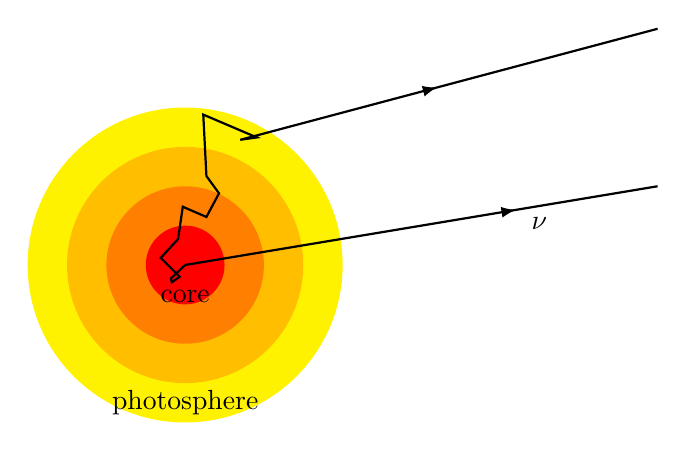
\begin{tikzpicture}[
  particle/.style={thick,decoration={markings, mark=at position .7 with {\arrow[>=latex]{>}}},postaction=decorate}
]
\fill[yellow] (0, 0) circle (2cm);
\fill[orange!50!yellow] (0, 0) circle (1.5cm);
\fill[orange] (0, 0) circle (1cm);
\fill[red] (0, 0) circle (.5cm);

\node at (0, -.4cm) {core};
\node at (0, -1.75cm) {photosphere};

\draw[particle] (0, 0) -- (6cm, 1cm) node[below,near end] {\Pneutrino};
\draw[particle] (0, 0)  -- (-0.18, -0.17)  -- (-0.17, -0.22)  -- (-0.07, -0.15)  -- (-0.31, 0.09)  -- (-0.09, 0.33)  -- (-0.03, 0.74)  -- (0.27, 0.61)  -- (0.43, 0.91)  -- (0.27, 1.13)  -- (0.23, 1.91)  -- (0.91, 1.62)  -- (0.70, 1.59) -- (6cm, 3cm) node[below,near end] {\Pphoton};
\end{tikzpicture}
\caption{Zonsdoorsnede} 
\label{fig:Zonsdoorsnede}
\end{figure}

In \figref{fig:Zonsdoorsnede} zie je een gamma en een neutrino de zon 
verlaten. Beide zijn ongeveer geproduceerd op hetzelfde moment. \\
    \begin{opdrachten} 
    \item Leg uit dat het neutrino de zon veel
    sneller zal verlaten dan het gamma. 
    \textit{het neutrino heeft
    (bijna) geen interactie met materie dus zal met ongeveer de
    lichtsnelheid door de zon gaan. Het gammafoton wordt keer op keer geabsorbeerd en
    weer uitgezonden door atomen in de zon. Voordat het foton het zonsoppervlak heeft bereikt,
    kunnen er wel een miljoen jaar verstreken zijn.}
    
    \item Zoek op in BINAS hoe groot het uitgestraald vermogen van de zon is. 
    \textit{Het uitgestraalde vermogen is } P = \SI{0.390e27}{\watt}.
    
    \item Bereken het aantal neutrino's dat de zon per seconde uitzendt.
    \textit{ We weten het vermogen van de zon en wat er per reactie aan energie vrijkomt.
    Per (`netto'-) reactie komen er twee neutrino's vrij.}

    \begin{eqnarray*}
    E_{reactie} = \SI{26.731}{\mega\electronvolt} *\SI{1.602e-13}{\joule \per\mega\electronvolt} \\
    E_{reactie} = \SI{4.2823e-12}{\joule}\\
    n = \frac{P}{E} = \frac{\SI{0.390e27}{\watt}}{\SI{4.2823e-12}{\joule}}\\
    n = 2* \SI{9.11e37}{} = \SI{1.82e38}{}
    \end{eqnarray*}
  
    
    \item Bereken de massavermindering van de zon in één jaar.
    \textit{ Het aantal reacties per s is \SI{9.11e37}{}. In één jaar zitten 
    \SI{3.15e7}{\second}. Per reactie wordt $\frac{\SI{26.731}{\mega\electronvolt}}{\SI{938.49}{\mega\electronvolt\per\atomicmassunit} }$
    = \SI{0.0285}{\atomicmassunit} omgezet. Dit is \SI{4.748e-29}{\kilo\gram} per reactie. 
    Dus aantal reacties per jaar:}
    \begin{eqnarray*}
    n_{reacties} = \SI{3.15e7}{\second}*\SI{9.11e37}{\per\second} \\
    n_{reacties} = \SI{2.87e45}{} \\
    m_{omgezetinéénjaar} = \SI{2.87e45}{} * \SI{4.748e-29}{\kilo\gram} = \SI{1.36e17}{\kilo\gram}
    \end{eqnarray*}
    
    
    Alle neutrino's verlaten de zon. Ze worden naar alle richtingen uitgezonden. 
    Op aarde is een neutrinodetector opgesteld met een naar de zon gekeerde 
    doorsnede van 5,0 m$^{2}$.\\
    \item Zoek op in BINAS hoe groot de afstand van de detector tot de zon gemiddeld 
    is. \\
    \textit{ De afstand van de aarde tot de zon is (gem.)} \SI{1.496e11}{\meter}
    
    \item Bereken hoeveel neutrino's per seconde de detector bereiken.
    \textit{ De geproduceerde neutrino's worden verdeeld over een boloppervlak met een straal van \SI{1.496e11}{\meter}.
    Voor het oppervlak van een bol geldt:} A = 4 $\pi r^{2}$.
    \begin{eqnarray*}
    A_{bol} = 4 \cdot \pi \cdot (\SI{1.496e11}{}) ^2\\
    A_{bol} = \SI{2.812e23}{\meter\squared}\\
    n_{neutrino's door detector} = \frac{5.0}{\SI{2.812e23}{}} * \SI{1.82e38}{}\\
    n_{neutrino's door detector} = \SI{3.2e15}{}
    \end{eqnarray*}   
    \end{opdrachten}

\end{opdrachten}
\end{document}
